\chapter{Introducción}

\section{Contexto y motivación}
En las últimas dos décadas, se ha incrementado el uso de la tecnología en la vida diaria, tanto como \textit{hardware} y \textit{software}. Una clara muestra de esto es la enorme cantidad de computadoras, celulares, consolas de vídeo juegos, cámaras de vídeo que existen en la actualidad y forman parte del día a día de las personas. También ha aumentado el numero de áreas donde la tecnología juega un papel protagónico o donde su aplicación se ha vuelto indispensable.

Una de estas áreas es la seguridad, y específicamente el área de vídeo vigilancia, donde su principal objetivo es monitorear instalaciones industriales estos sistemas de vigilancia son conocidos como \ac{CCTV} y aún son usados desde espacios públicos hasta edificios privados y hogares. Y su difusión ha ido aumentando con el paso del tiempo por el menor costo del \textit{hardware} y la mayor preocupación por un control de seguridad. Esta mayor preocupación motiva la investigación de técnicas que nos permita identificar a las personas sin su cooperación, sobretodo en escenarios como la identificación de personal autorizado, verificación de pasaporte, control de acceso, vigilancia de multitudes en estaciones, áreas publicas, etc.
%%\cite{bolme2003elastic}.

Por ello se ha difundido el uso de técnicas biométricas para el reconocimiento de individuos. Para que una forma de reconocimiento pueda considerarse biométrica tiene que cumplir los siguientes requerimientos; Universalidad: Cada persona debe tener las características que se usan para el reconocimiento, Distintividad: Cualquier par de personas deben ser lo suficientemente diferentes en términos de las características, Permanencia: Las características deben ser lo suficientemente invariantes (con respecto a la forma de comparación) en un periodo de tiempo, Adquisición: Las características deben ser medidas de forma cuantificable.%agregar referencia a paper de biometria
Muchas de estas técnicas se basan en imágenes como las misma huellas dactilares, el iris de los ojos, la geometría de las palmas y el rostro. 

El reconocimiento biométrico de individuos a partir del rostros se realiza a partir de imágenes las cuales pueden ser estáticas (fotografías) o dinámicas (imágenes de vídeo vigilancia). En el caso de la vídeo vigilancia se toma en cuenta el hecho que no se tiene control sobre varios factores que influye en proceso de reconocimiento como la iluminación, el angulo de visión, y otros factores que se explicaran con más detalle más adelante, mientras que otros métodos de reconocimiento biométrico no presentan dichas dificultades por la forma de adquisición de los datos.

%ya no es necesario hablar de paralelo
%Estas ultimas producen un mayor volumen de información para ser tratadas y obtener un resultado en tiempo real, por ello se considera el uso del paralelismo masivo, siendo una tendencia en los últimos años la implementación de algoritmos para ser masivamente paralelos.

Según el \textit{survey} de la literatura de Zhao \cite{zhao2003face}, los métodos de reconocimiento de rostros se pueden clasificar mediante el enfoque en por el cual aborda el problema, es decir como tratan a la imagen del rostro. En la Figura \ref{im:métodos} podemos ver algunos algoritmos clasificados por enfoque. Siendo algunos de los más conocidos \acf{LDA}, \acf{PCA}, \acf{EBGM} \cite{zhao2003face}.

\begin{figure}[h]
\center
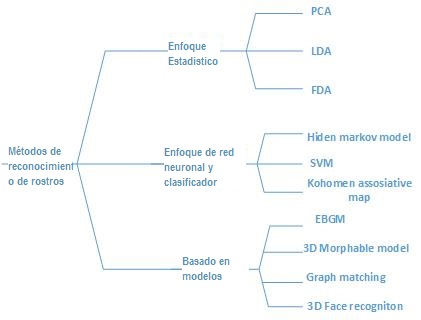
\includegraphics[scale=1]{Metodos}
\caption{Clasificación de métodos de reconocimiento de rostro por enfoque.}
\label{im:métodos}
\end{figure}

Según la Figura \ref{im:métodos} los métodos de reconocimiento de rostros pueden ser agrupados en métodos holísticos y métodos basados en características \cite{tseng2003comparison}, y según Zhao \cite{zhao2003face} podemos agregar los métodos basados en Inteligencia artificial.

Los métodos holísticos tratan a la imagen como un todo, donde la extracción de características depende de la variación total de la información que conforma la imagen, por esta razón no sabemos que características se extraen ni podemos darles una jerarquía de valores, por esta razón son sensibles a cambios de iluminación y fondo.

Los métodos basados en características, como lo dice su nombre se basan en formas localizadas de extracción de características donde si se tiene el conocimiento de cuales son y puede aplicarse un orden de importancia a ellas, generalmente el reconocimiento se realiza mediante una forma de distancia entre las características de dos diferentes imágenes.

Agregando a estas dos formas se considera el enfoque basado en inteligencia artificial donde en vez de tener un medida de distancia simple el reconocimiento se realiza a través de un clasificador o otro método basado en inteligencia artificial.

%\ac{PCA} es un método para la reducción de la dimencionalidad sin supervisión \cite{sirovich1987low} \cite{turk1991eigenfaces}.Que toma le rostro como un todo, extrayendo sus características lineales, es uno de los algoritmos más populares, que ha sido usado extensivamente, y continua su investigación y mejora.

%\acf{EBGM} es un método que puede extraer información de puntos biométricos del rostro también conocidos como puntos fiduciales a diferencia de los métodos de enfoque estadístico que tratan a la imagen como un todo o las redes neuronales que dependen del entrenamiento que se les proporciones. Este método será explicado con mayor detalle en los siguientes capítulos.


\section{Planteamiento del problema}

El reconocimiento de rostros en  presenta muchos problemas los cuales aún persisten o no han sido resueltos en su conjunto y totalidad por algún método o algoritmo ya existente, estos problemas son listados a continuación:

\begin{enumerate}[1.]
\item Efectos de la iluminación \cite{kalocsai1998face} \cite{gross2001quo} \cite{johnston1992recognising} \cite{bruce1998human} \cite{hill1996effects}.- Debido a que un rostro es un objeto 3D, las fuentes de luz indirectas puedes causar grandes sombras que acentúan o disminuyen ciertas características faciales. Los efectos de la iluminación en las imágenes se puede deber a la cantidad inherente de luz reflejada en la piel y a los ajustes no lineales dentro de la cámara. Todo ello afecta a la calidad de la imagen o vídeo \cite{chiang1997local} \cite{aizawa1992scheme}.
\item Variación según el punto de visión  \cite{hill1997information} \cite{gross2001quo}.- El rostro es un objeto  3D y debido al ángulo de visión de la cámara la apariencia del rostro puede variar debido a la deformación proyectiva, la cual lleva a que la parte inferior de rostro se vea más angosta de lo que realmente es.
\item Expresión\cite{gross2001quo}.-  El rostro es un objeto no rígido, las expresión de la emociones y parte de la comunicación paralingüistica junto con el habla, y la variación de esas expresiones faciales influye en el reconocimiento de de el rostro.
\item \textit{Time delay} \cite{gross2001quo}.- Es el intervalo de tiempo entre la adquisición de la imagen que se desea reconocer y la imagen o los datos con los cuales realizamos la identificación por ejemplo, intentar identificar a un sujeto el cual su ultima fotografía fue tomada hace un año.
\item Factores individuales\cite{gross2001quo}.- Se considera factores individuales a aquellos como el uso de maquillaje, estilos de peinado, disfraces, y otras formas en las que las personas modifican su apariencia
a gusto personal.
\item Oclusión.- La oclusión puede darse debido a objetos en la escena o al uso de lentes de sol y otros objetos, también debido a la falta de cooperación de los individuos y a la variación según el punto de visión.
\item Las imágenes de los  rostros son pequeños.- Debido a las condiciones de adquisición, las imágenes de los rostro son más pequeñas y de menor calidad de lo que asumen la mayoría de los sistemas de reconocimiento de rostros existentes. Por ejemplo, una región de rostros valida puede ser tan pequeña como 20$\times$20 pixeles, mientras los tamaños de las imágenes de los rostros usados en los sistemas actuales son tan grandes como 128$\times$128. El pequeño tamaño no solo hace la tarea de reconocimiento difícil, también afecta la precisión de la detección de los puntos de marca que a menudo son necesarios en los métodos de reconocimiento.
\item Las características de los objetos rostro/humano \cite{zhao2003face}.- El rostro humano como objeto es fácil de reconocer si se compara con otro objeto que no sea un rostro (diferencia Inter-clase) pero resulta mas difícil de reconocer si se le compara con otro rostro (diferencia Intra-clase) por ello detectar y localizar rostros es mucho más fácil que reconocer un rostro en especifico. Por ello el reconocimiento es un tarea más complicada debido a que se realiza un trabajo de detección previo, sobre todo si es en vídeo vigilancia.

\end{enumerate}


\section{Objetivos}
Escoger de la literatura el método más apropiado para el contexto de vídeo vigilancia y analizar dicho método.

\subsection{Objetivos específicos}
%Como objetivos específicos tenemos:

%To increase the success rate in EGBM we prove the following parameters:
%Model Increment
%Weighted Similarity Function.
%Illuminations enhancement.
%Gabor Wavelet size.
%Landmark localization.

\begin{itemize}
\item Establecer los métodos de reconocimiento de rostros en la literatura.
\item Realizar el comparativa con los métodos mas usados en la literatura.
\item Escoger un método y analizarlo para su uso en el contexto de vídeo vigilancia.
\item Probar el método escogido con datos reales de vídeo vigilancia. 
%\item Implementar el metodo de reconocimento para pruebas.
%\item Convertir el metodo de reconocimiento de rostros masivamente paralelo.
%\item Probar con imagenes de video vigilancia
%\item Analizar los resultados
\end{itemize}


\section{Organización de la tesis}

En los próximos capítulos se desarrollará el trabajo que comprende toda la tesis, en esta sección realizaremos una breve descripción de ellos.

En el Capítulo 2 presentamos varios conceptos que se relacionan con nuestra propuesta, como son las técnicas de reconocimiento que usamos. Todo ello con el fin de hacer entendibles las menciones de dichos conceptos en el resto del trabajo.

En el Capítulo 3 describiremos brevemente los trabajos que se relacionan de algún modo con reconocimiento de rostros, agrupándolos en relación \ac{EBGM}, que es nuestro método escogido.

En el Capítulo 4 exponemos nuestra propuesta con la cual pretendemos alcanzar el objetivo presentado en este capítulo.

En el Capítulo 5 mostraremos los resultados de la pruebas realizadas

Y finalmente exponemos nuestras conclusiones finales.